
\chapter{Validierung}

\section{Analyse der spannkraftinduzierten Deformation}\

[explizit Unterschiede FDM und additiv herausstellen mit genauen Angaben über die Deformationen]

Mithilfe dieser Funktion können unterschiedliche Bauteilgeometrien und
Herstellungsprozesse auf ihre Deformation hin verglichen werden.
Bei einem additiv gefertigten Metallteil tritt bei den 
gleichen Spannungsstufen eine deutlich kleinere, 
aber dennoch erkennbare Deformation auf. Zusätzlich zeigt sich, 
dass bei verschiedenen Herstellungsprozessen trotz gleicher 
Geometrie unterschiedliche Verformungen auftreten.
Die verschiedenen Verformungen und Auswirkungen werden später in diesem
Kapitel behandelt.

\begin{figure}[H]
    \centering
    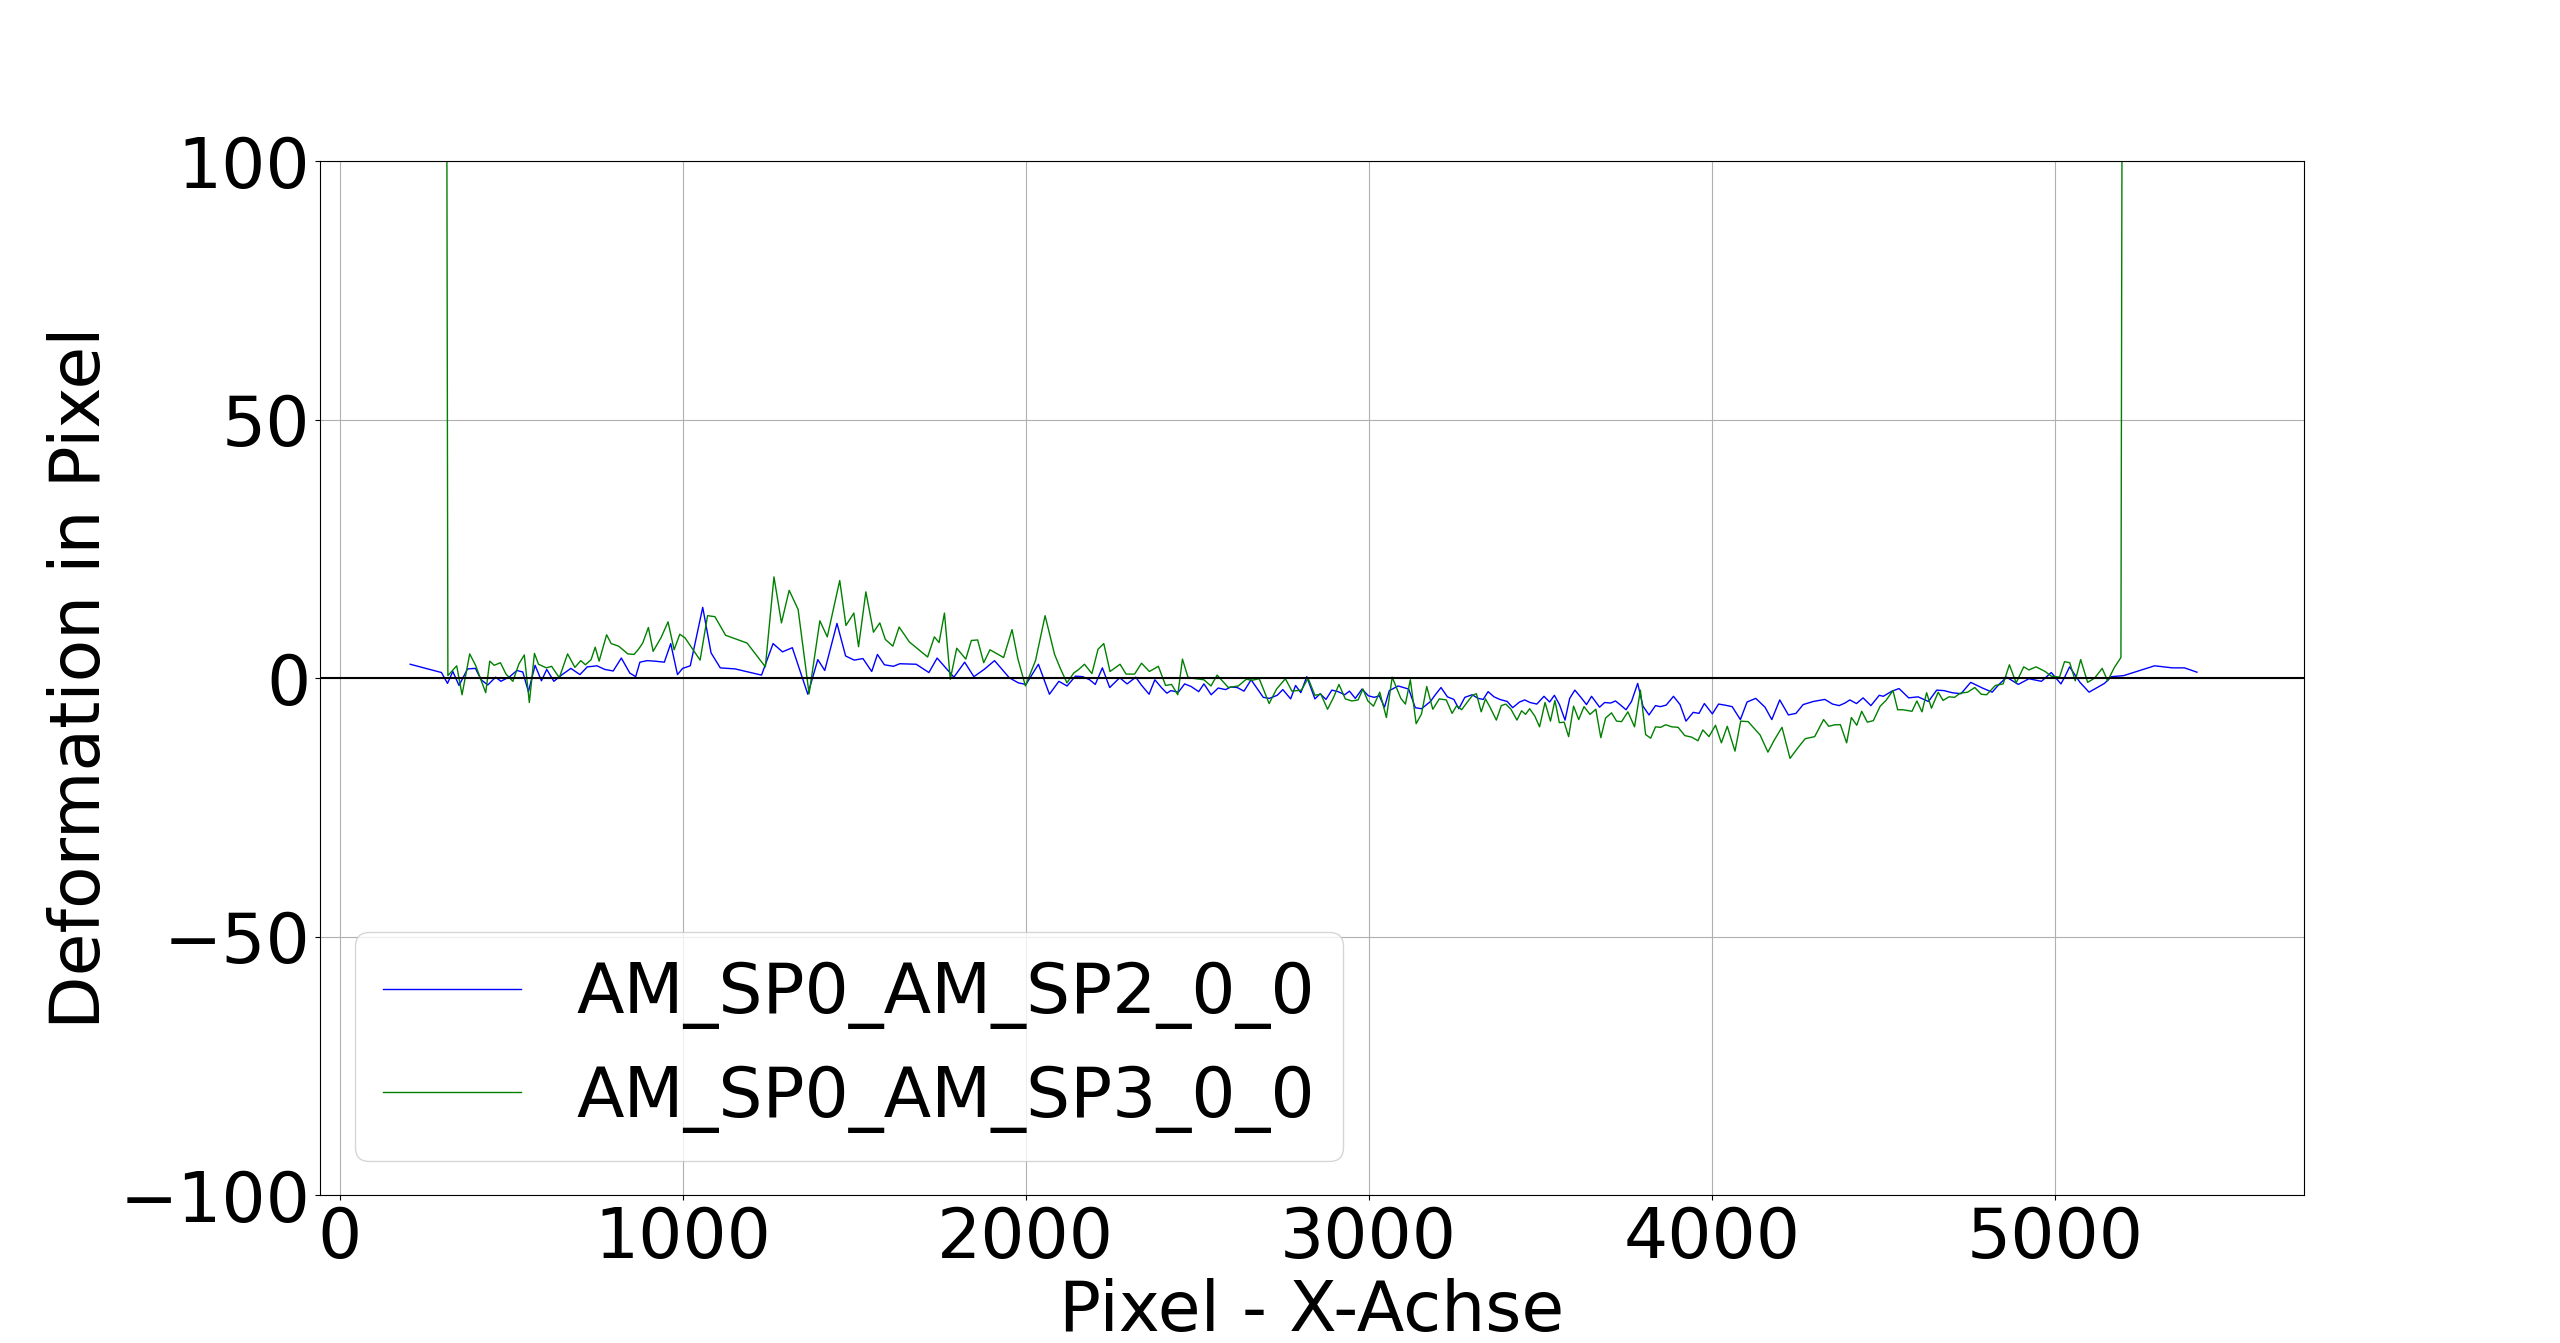
\includegraphics[width=0.9\textwidth]{images/AM_sp0_sp2_defo_plot.png}
    \caption{Differenz von mehreren Spannungsstufen bei einem AM Metall Bauteil}
    \label{fig:deformation_data_am}
\end{figure}

\section{Messergebnisse}

Es wurden fünf Bauteile mit verschiedenen Spannungsstufen gemessen. Für jede 
Spannungsstufe wurde die Kraft, die auf das Bauteil wirkte sowie die Verschiebung 
des Schraubstocks gemessen.
Jede Spannungsstufe wurde durch Stufenweises anziehen des Schraubstocks erreicht.
Die Spannkraftkurve eines einzelnen Einspannvorgangs ist in 
Abbildung \ref{fig:single} zu sehen. 
In der Spannungskurve ist ein elastischer Bereich für das 
Bauteil zu sehen, in dem sich die Spannkraft zurückbewegt, nachdem kein 
Anzugdrehmoment mehr anliegt. Aus diesem Grund kann nicht der maximale Wert der Spannkraft angenommen werden, 
sondern es muss ein Wert gewählt werden der nach dem maximalen Ausschlag liegt.
Dieser wurde über die erste Ableitung der Spannkraftkurve gefunden. Sobald der 
Absolutwert der Steigung unter 0.0009 N fällt, wir die Spannkraft und Auslenkung an 
diesem Punkt gewählt. 0.0009 N wurde empirisch ermittelt, um bei allen Bauteilen einen 
angemessenen Wert zu liefern.
Die Spannkraft wurde an zwei Achsen aufgenommen und zu der Gesamtkraft aufsummiert.

\begin{figure}[H]
    \centering
    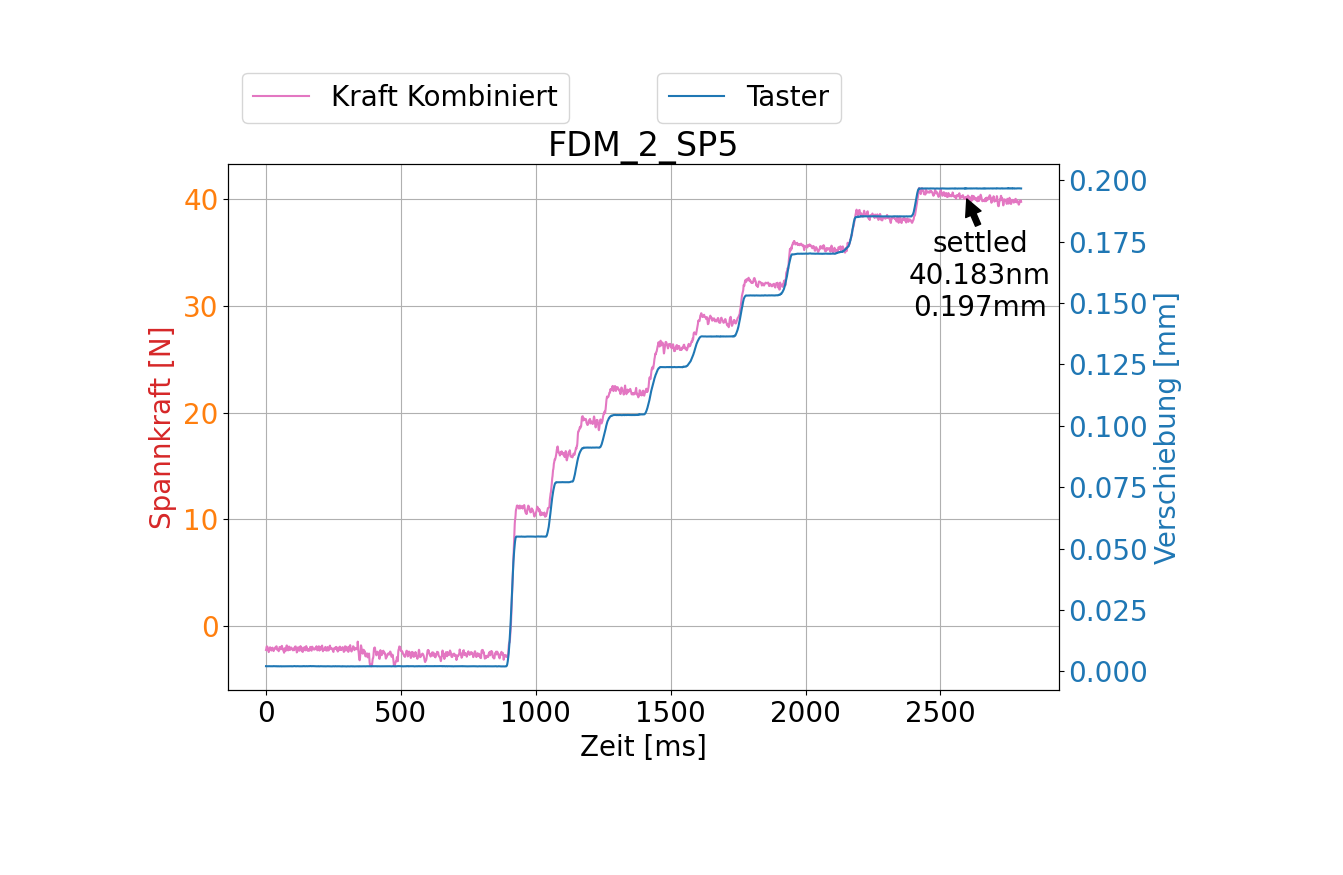
\includegraphics[width=0.99\textwidth]{images/spannkraftstufen_single.png}
    \caption{Kraft- und Verschiebung der Spannungsstufe fünf bei einem FDM Bauteil}
    \label{fig:single}
\end{figure}

Diese maximalen Werte für die Spannkraft und Auslenkung wurden für jedes Bauteil 
akkumuliert und sind in Abbildung \ref{fig:akkumulated} dargestellt. 
Die mit dem FDM-Prozess hergestellten Bauteile wurden jeweils in sechs Spannungsstufen
gemessen. Zwischen den Stufen wurde versucht, eine konstante Kraft auf das Bauteil 
auszuüben. Durch den manuellen Prozess des Anziehens des Schraubstocks war dies 
jedoch nicht immer möglich.
Die Metallbauteile unterscheiden sich durch ihren Aufbau. 
Alle basieren auf dem gleichen 3D-Modell, besitzen jedoch unterschiedliche 
Stützstrukturen. Im Bauteil AM0 ist die vollständige Stützstruktur vorhanden,
während in den Bauteilen AM1 und AM2 die Stützstruktur in unterschiedlicher 
Tiefe ausgebohrt wurde. Die Bauteile sind in Abbildung \ref{fig:am_parts} dargestellt.

Das Bauteil AM0 wurde nur mit zwei Spannungsstufen gemessen, 
da bereits bei der zweiten Stufe über 2500 N Kraft erforderlich war, 
um das Bauteil nur minimal in x-Richtung zu deformieren. Dies zeigt, 
dass die Stützstruktur einen erheblichen Einfluss auf die Verformbarkeit 
eines Bauteils hat. Beim Bauteil AM1 wurden 2500 N erst nach vier Spannungsstufen 
erreicht. Vergleicht man die Verformung in x-Richtung mit der Verformung von AM2,
 zeigt sich, dass das Bauteil ohne Stützstruktur bei ähnlicher Krafteinwirkung 
 etwa doppelt so weit in x-Richtung deformiert wurde.

 Die FDM-Bauteile wurden mit deutlich weniger Kraft eingespannt. 
 Hier wurde bei etwa 250 N gestoppt, dennoch ist die Verschiebung der 
 Teile deutlich größer als bei den AM-Bauteilen. Diese Werte wurden aufgenommen, 
 um die visuelle Deformationserkennung zu validieren.

\begin{figure}[H]
    \centering
    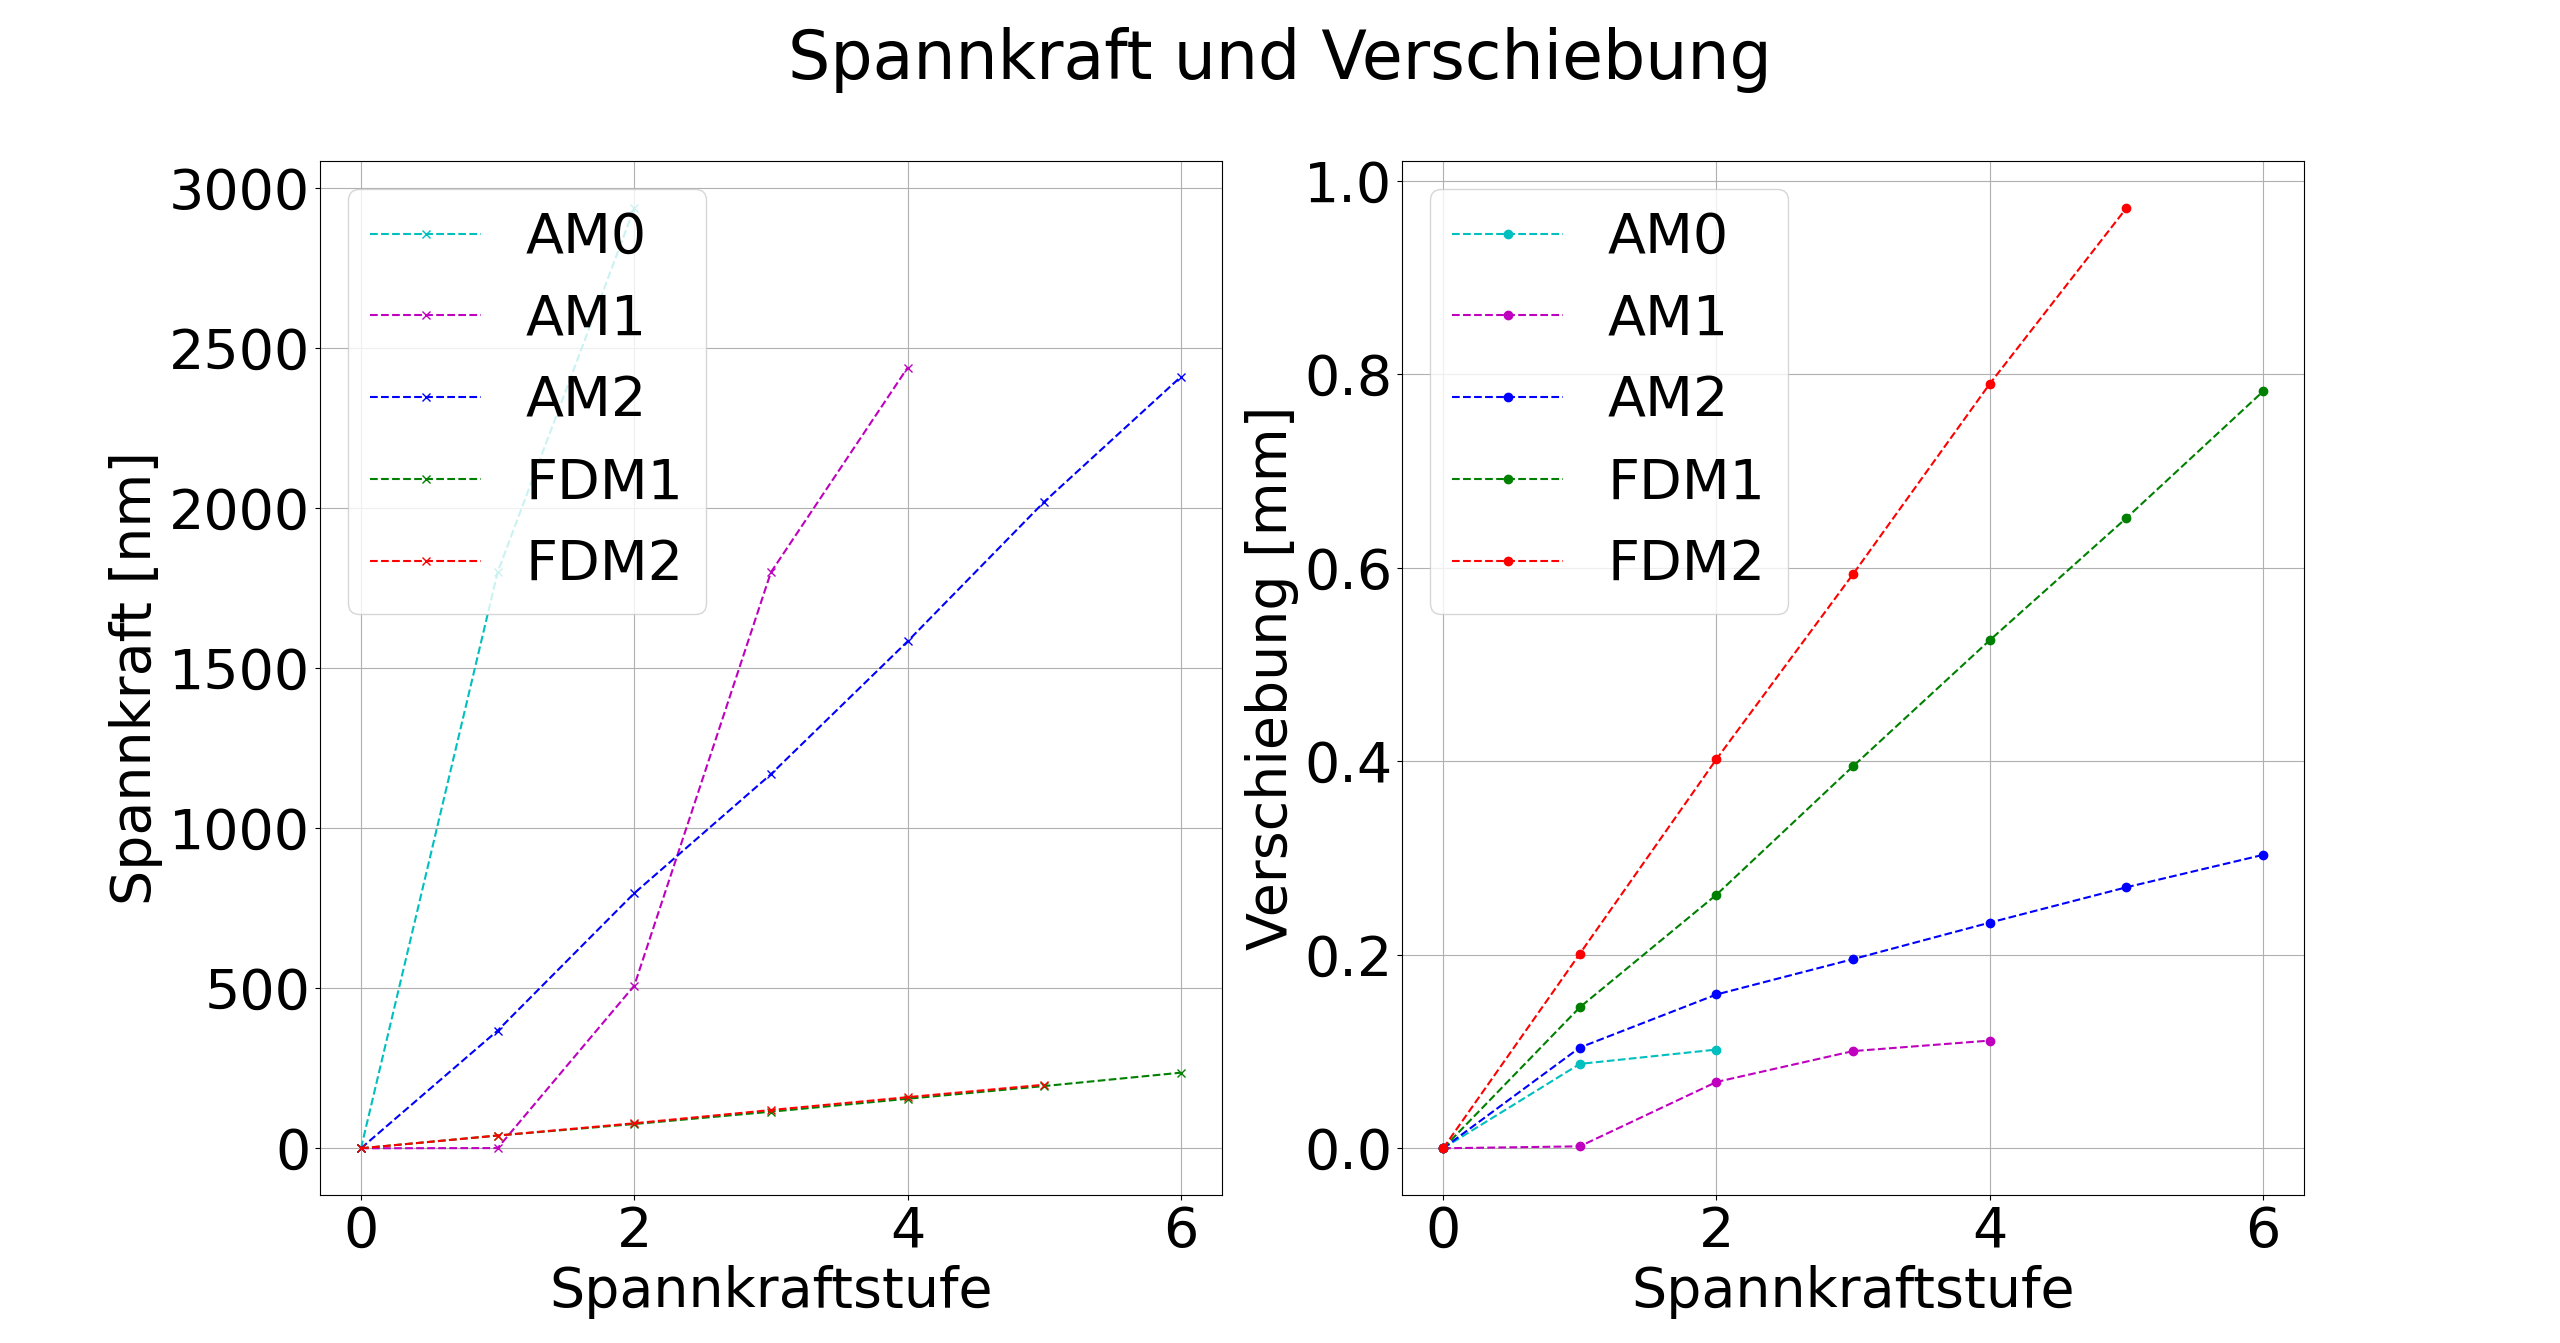
\includegraphics[width=0.99\textwidth]{images/spannkraftstufen_akkumuliert.png}
    \caption{Akkumulierte Kraft- und Verschiebung jedes Bauteils}
    \label{fig:akkumulated}
\end{figure}

\begin{figure}[H]
    \centering
    \begin{minipage}{.33\textwidth}
      \centering
      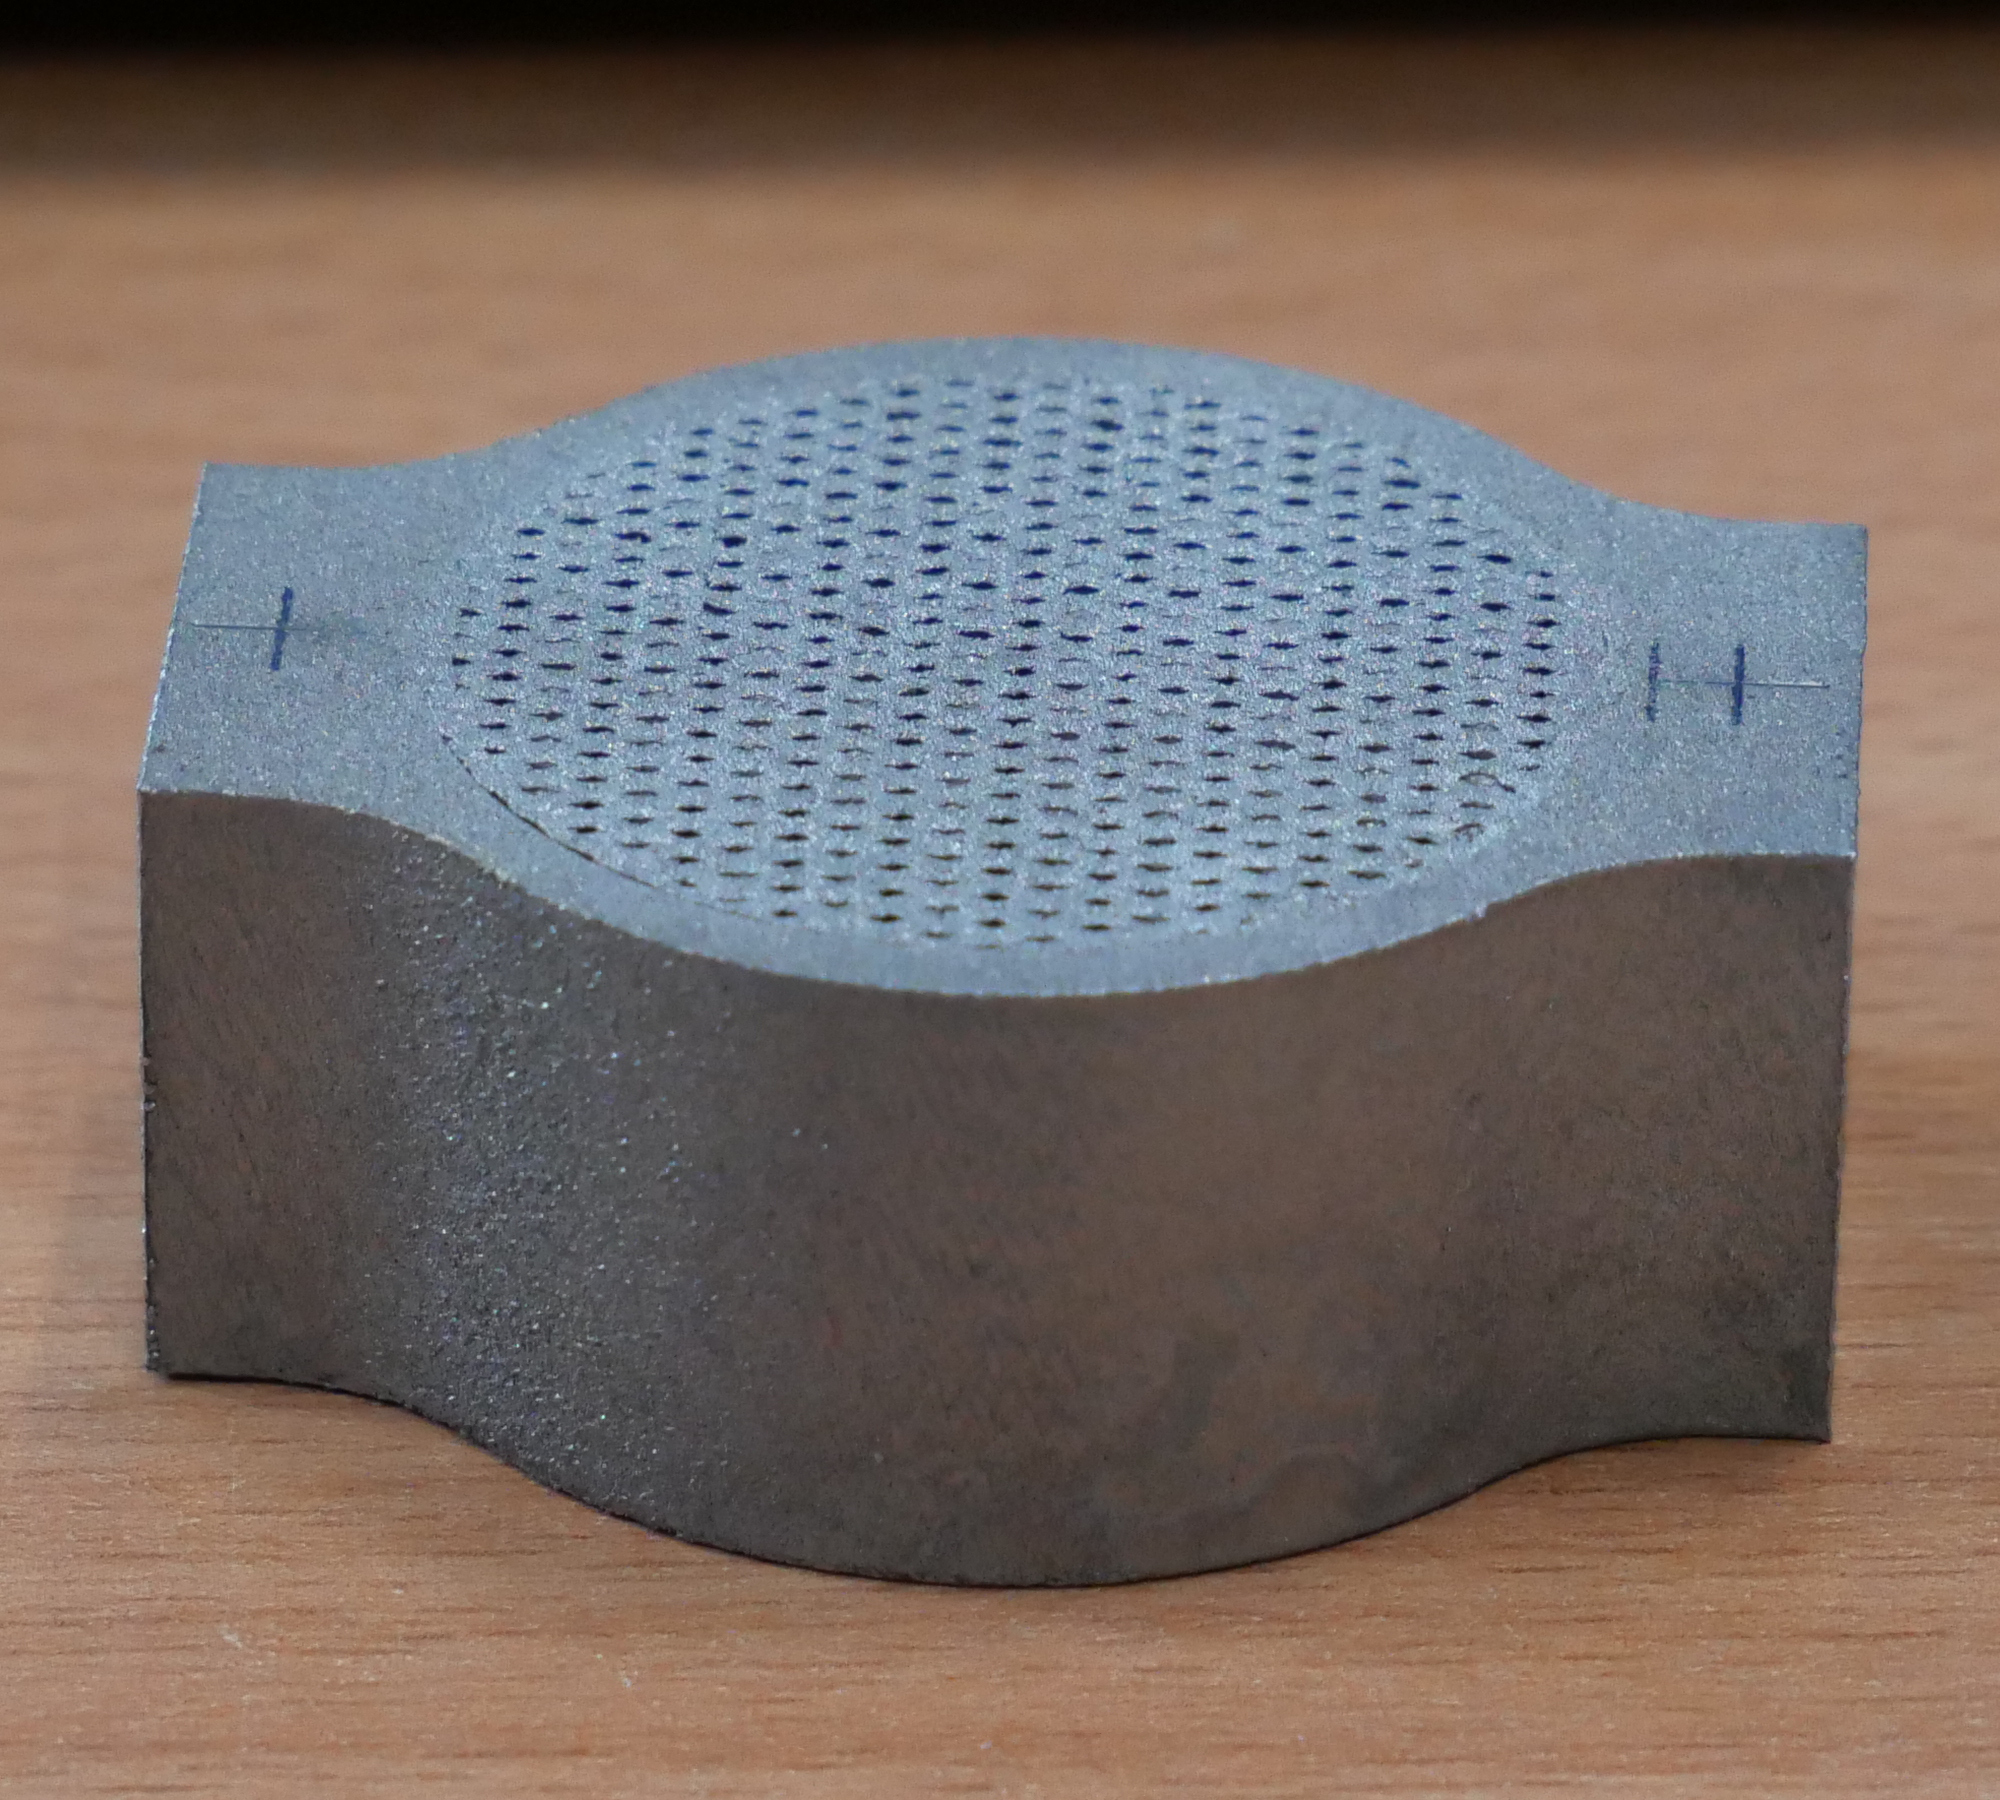
\includegraphics[width=0.9\linewidth]{images/AM0_crop.JPG}
      \caption*{(a)}
    \end{minipage}%
    \begin{minipage}{.33\textwidth}
      \centering
      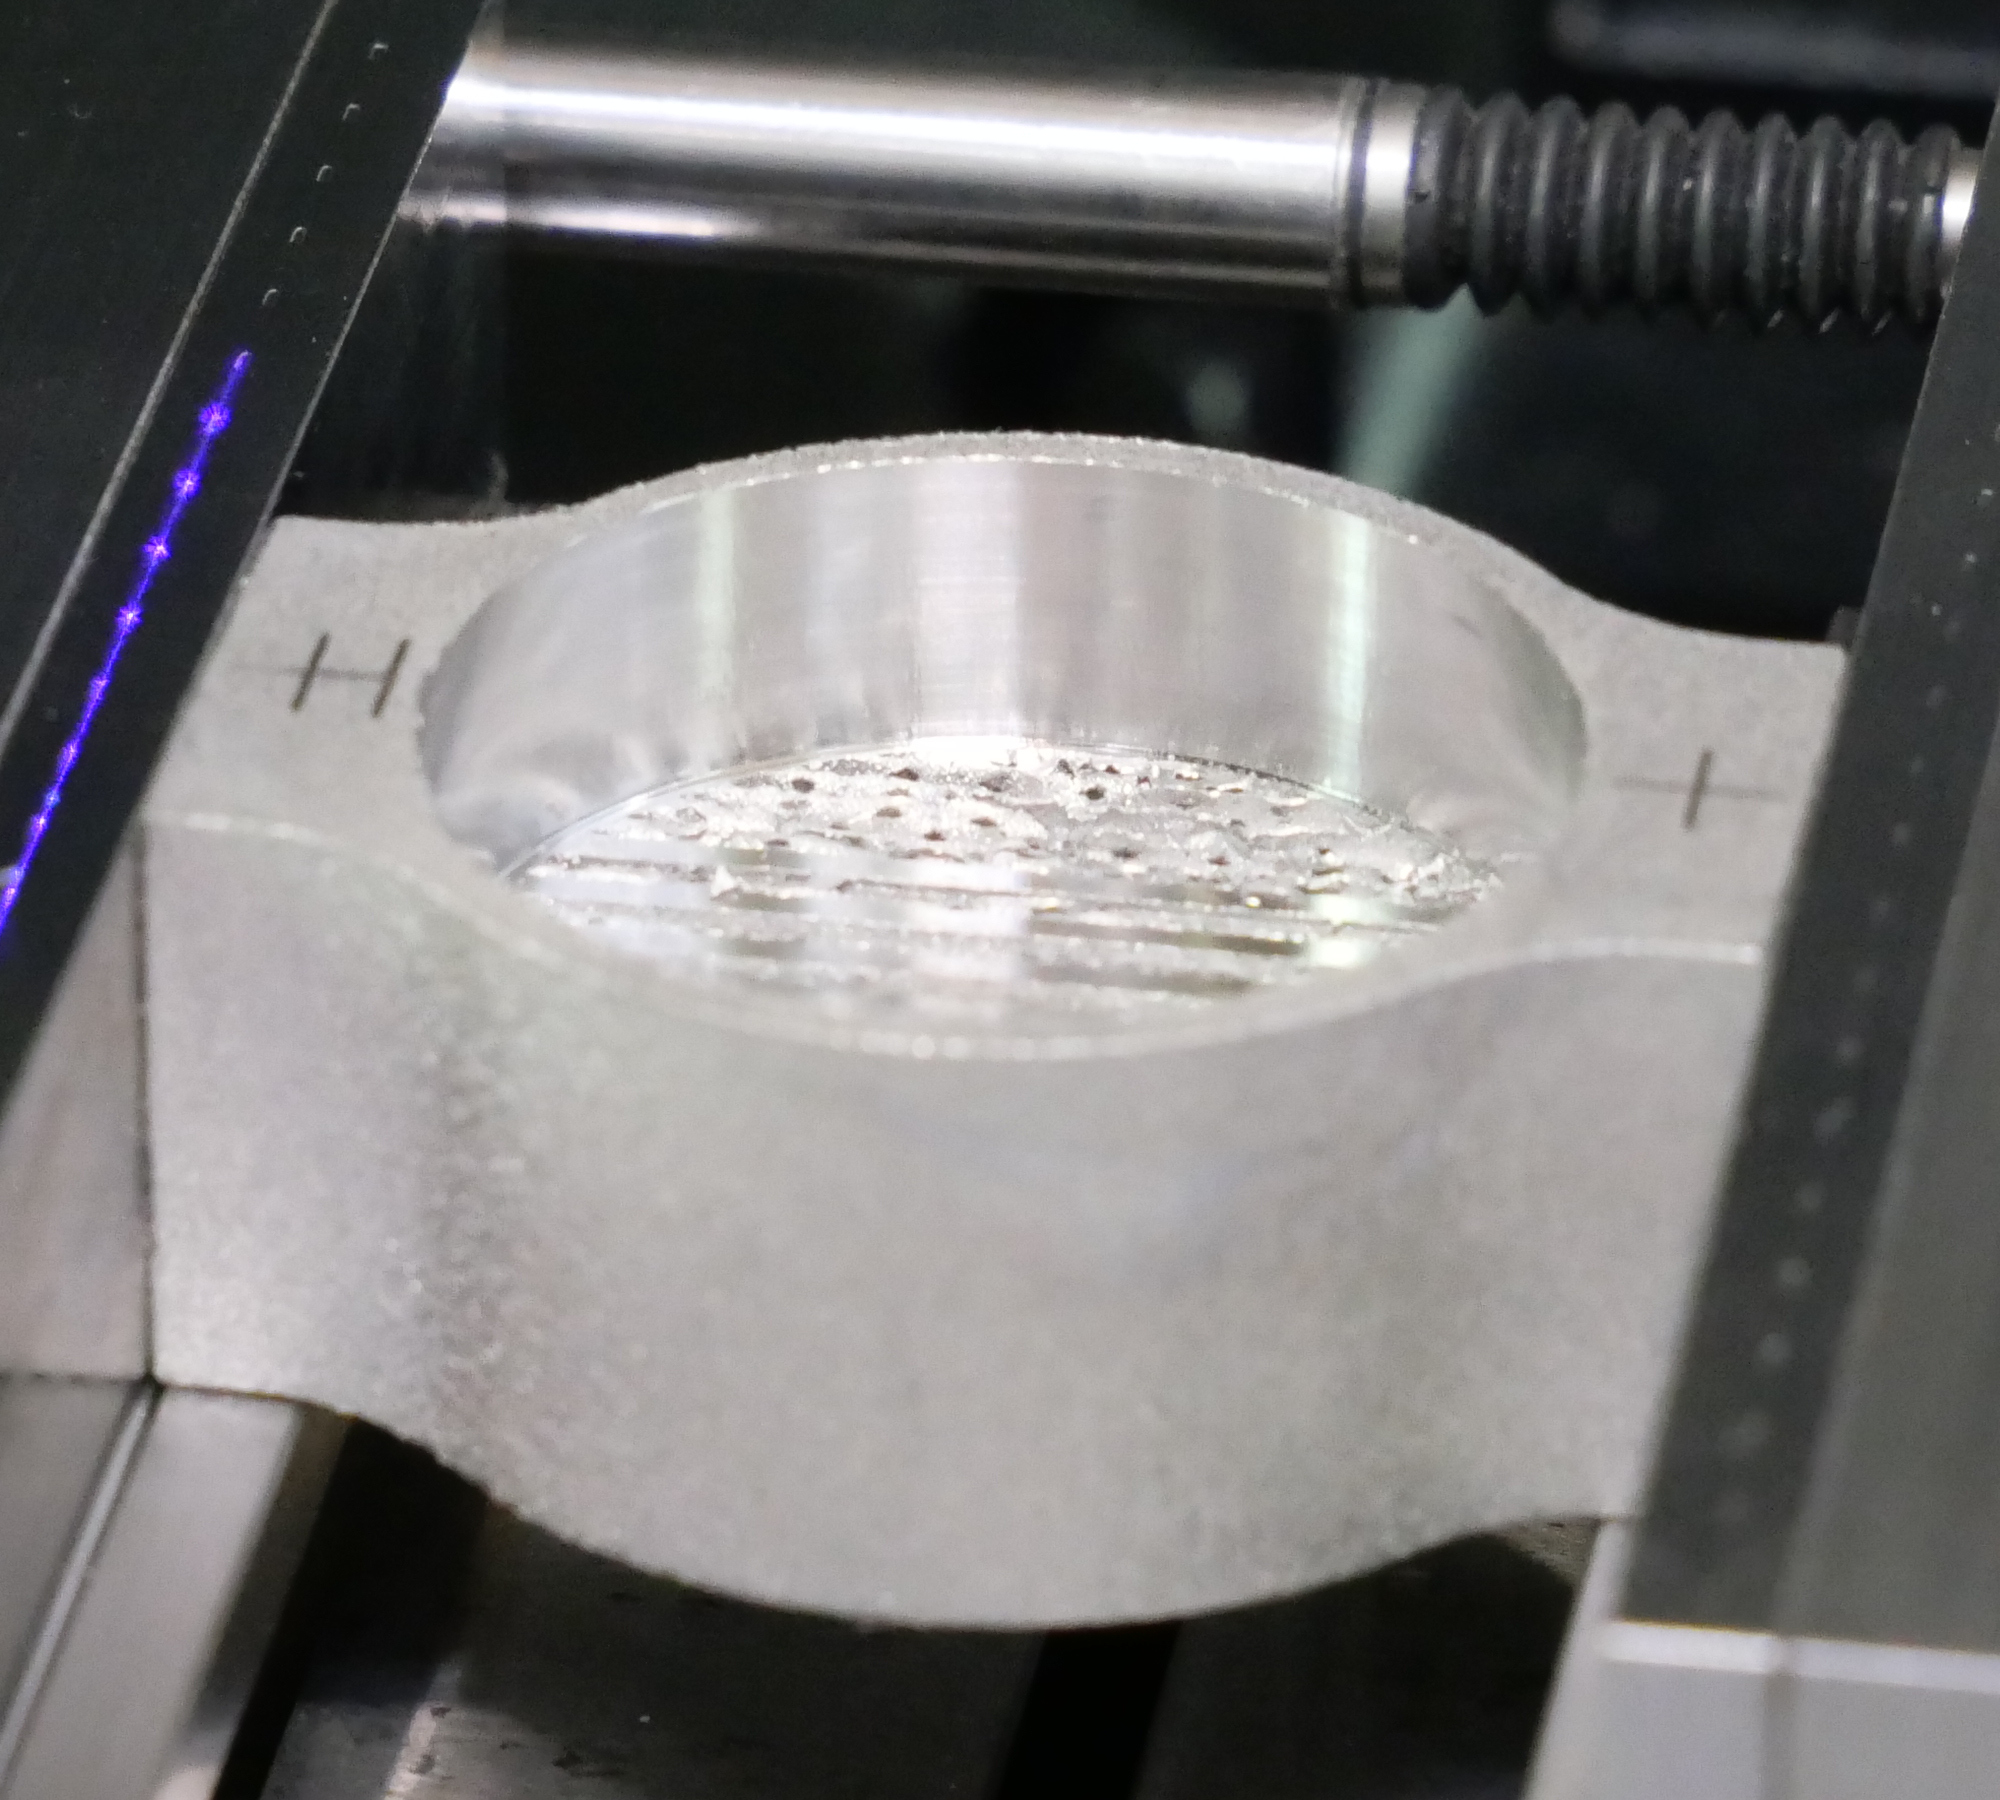
\includegraphics[width=0.9\linewidth]{images/AM1_crop.JPG}
      \caption*{(b)}
    \end{minipage}
    \begin{minipage}{.33\textwidth}
        \centering
        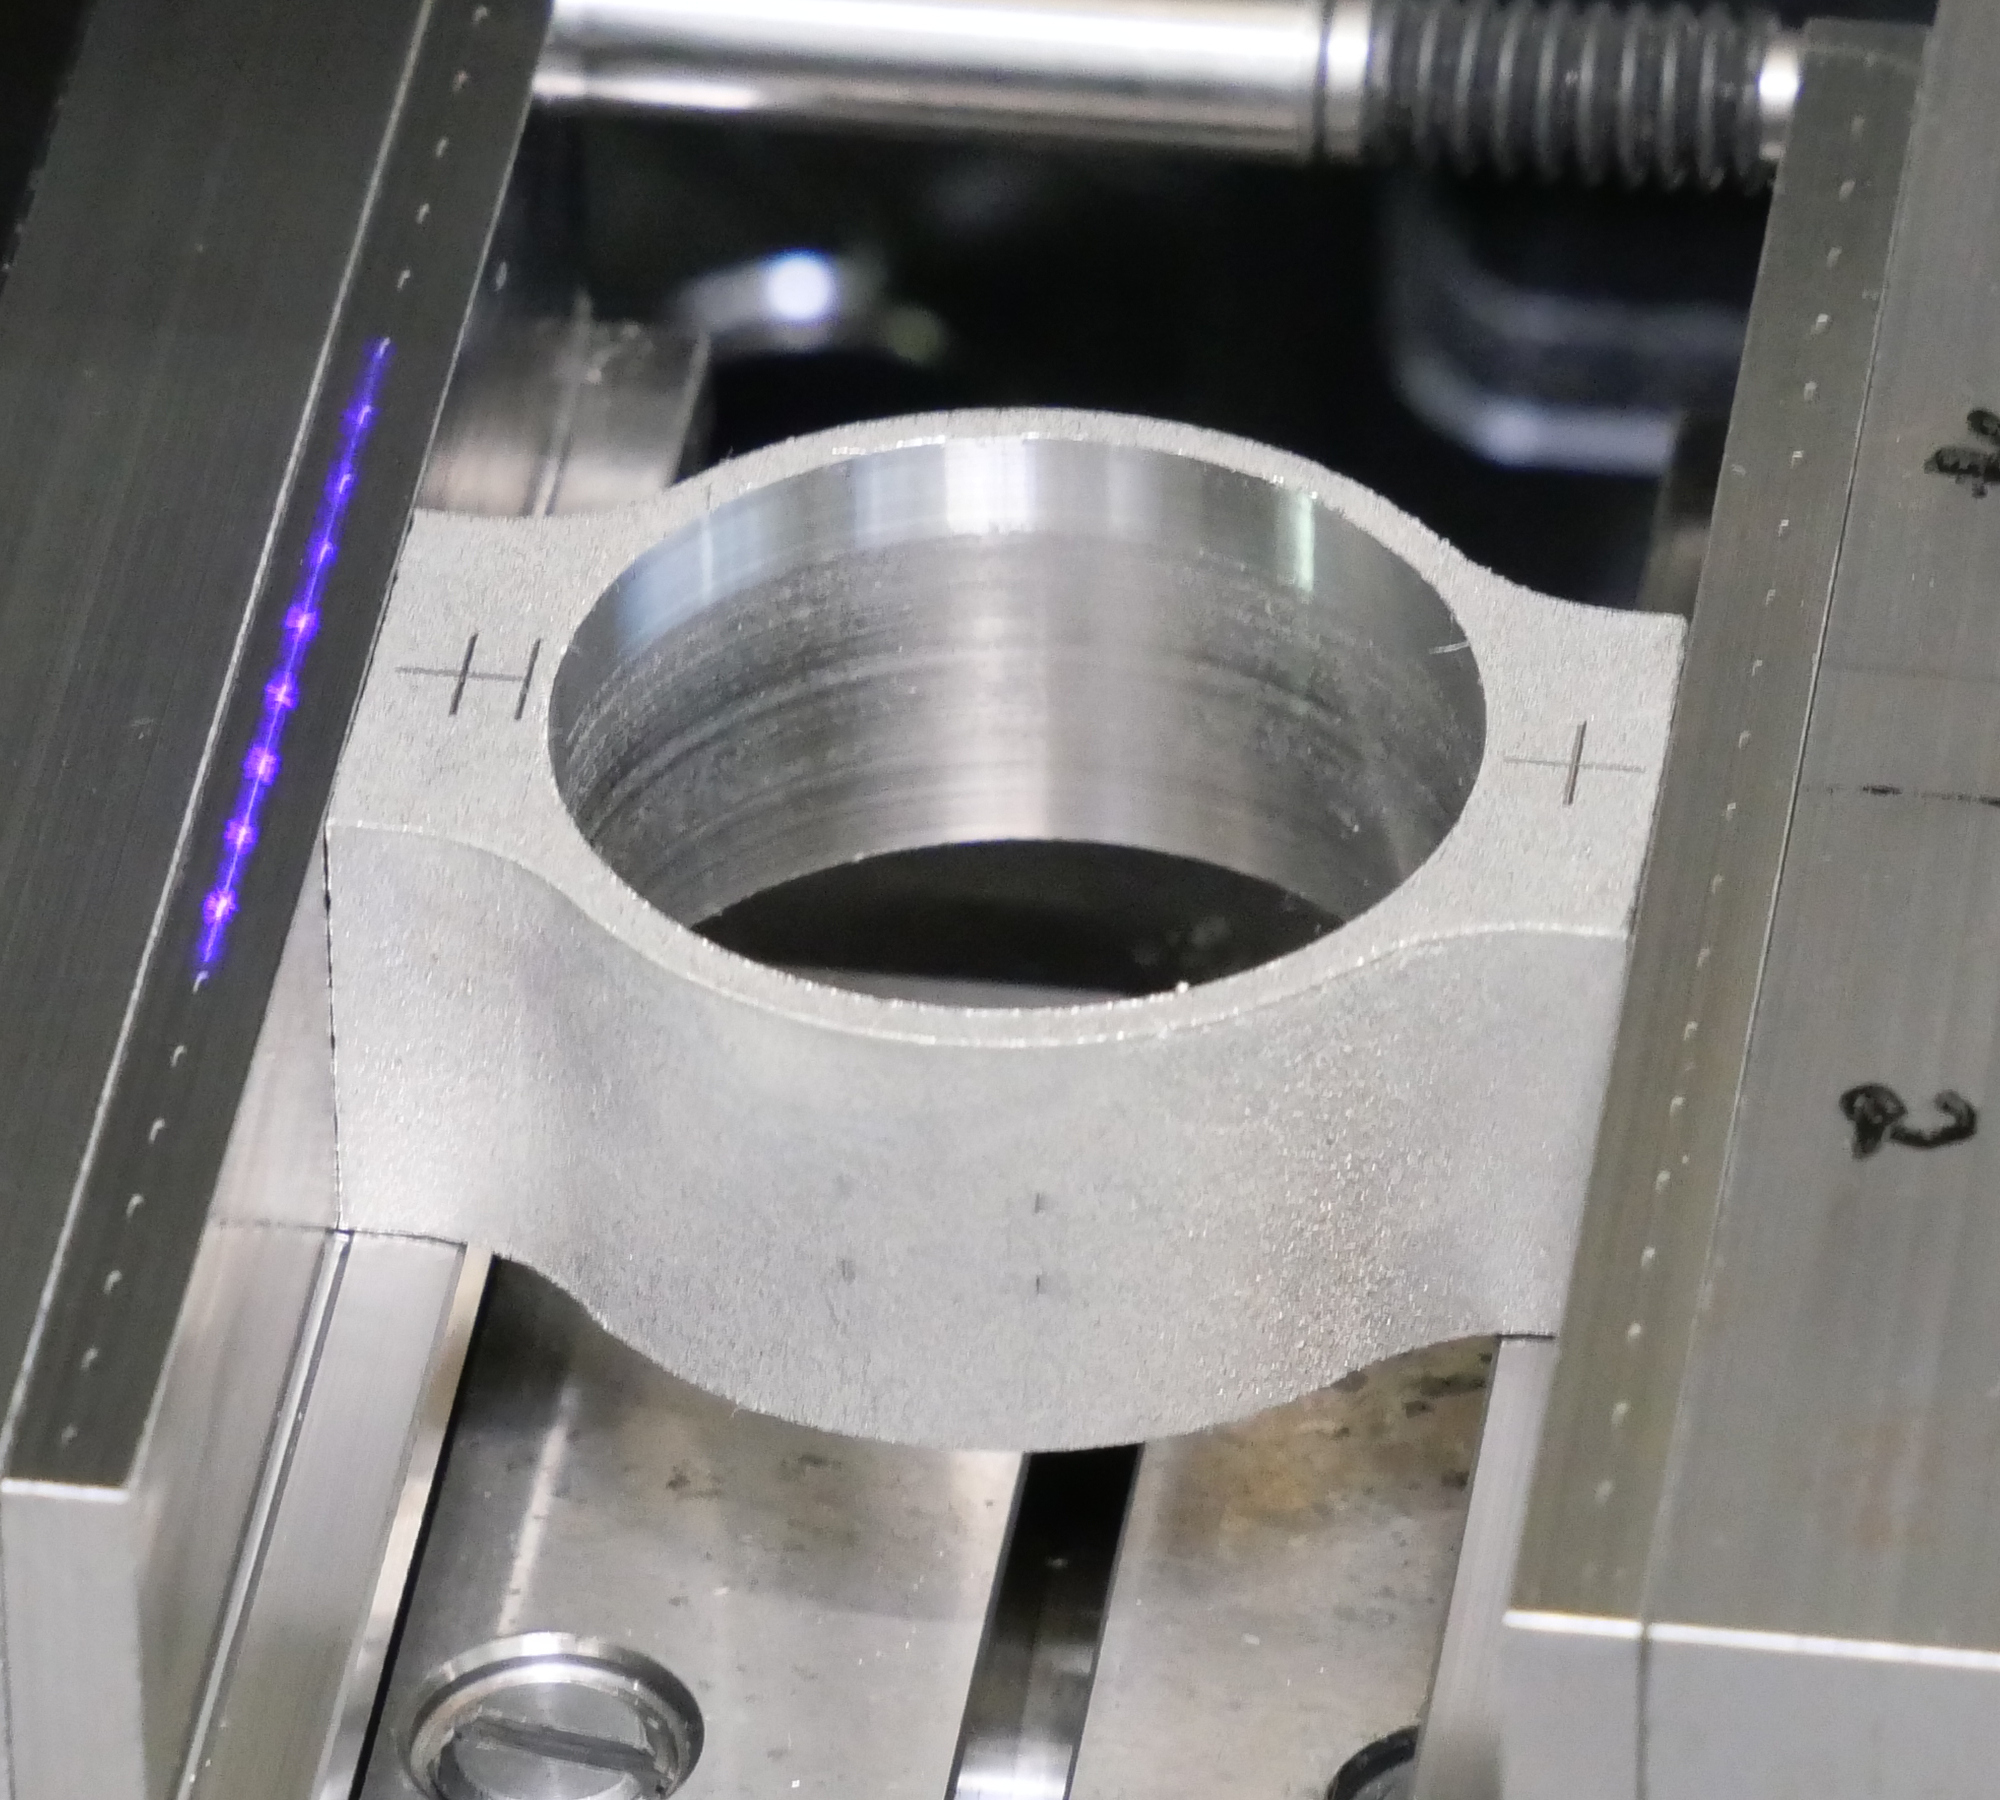
\includegraphics[width=0.9\linewidth]{images/AM2_crop.JPG}
        \caption*{(c)}
      \end{minipage}
      \caption{(a): AF Metallbauteil mit voller Stützstruktur, Bezeichnung: AM0.
      (b): AF Bauteil mit der halben Stützstruktur ausgebohrt, Bezeichnung: AM1.
      (c): AF Bauteil ohne Stützstruktur, Bezeichnung: AM2}
      \label{fig:am_parts}
\end{figure}

\section{Ergebnisse der optischen Deformationsanalyse}

In Abbildung \ref{fig:am_defos} und Abbildung \ref{fig:fdm_defos} sind die erkannten,
vertikalen Deformation grafisch dargestellt. Jeweils von Spannungsstufe null bis 
Spannungsstufen Sechs. Bei dem FDM Bauteil fehlt die Spannungsstufen fünf, 
diese ist leider bei der händischen Dateiname Vergabe überschrieben worden und konnte 
deshalb nicht ausgewertet worden. Aus diesem Grund ist eine so große Lücke in der 
Abbildung \ref{fig:fdm_defos}.
Außerdem sind große Unterschiede in der absoluten Deformation zu sehen. Zum Beispiel 
die rote Kurve in Abbildung \ref{fig:am_defos} die den Unterschied der Spannungsstufen 
null und eins angibt. Diese Kurve sollte näher an null der y-Achse liegen. 
Dies liegt an Ungenauigkeiten in dem Stitching Verfahren. In den Graphen ist also 
auf die Steigung der Deformationskurve zu achten. In der Steigung erkannt man das 
sich die Bauteile in mittleren Bereich nach außen hin deformiert haben und in 
den Randbereichen sich nach innen und dann wieder nach außen deformieren.
Außerdem ist im Vergleich der beiden Graphen zu sehen das sich das FDM Bauteil deutlich 
mehr verformt hat. Hier beträgt die größte Deformation über 150 Pixel.
Bei dem Metallbauteil, das mit der zehnfachen Kraft eingespannt wurde (250 nm vs. 2500 nm)
sind es nur knapp 40 Pixel. Trotzdem ist zu sehen das sich die Bauteile, die auch die 
gleiche Geometrie teilen, auf die gleiche Weise verformt haben.

\begin{figure}[H]
  \centering
  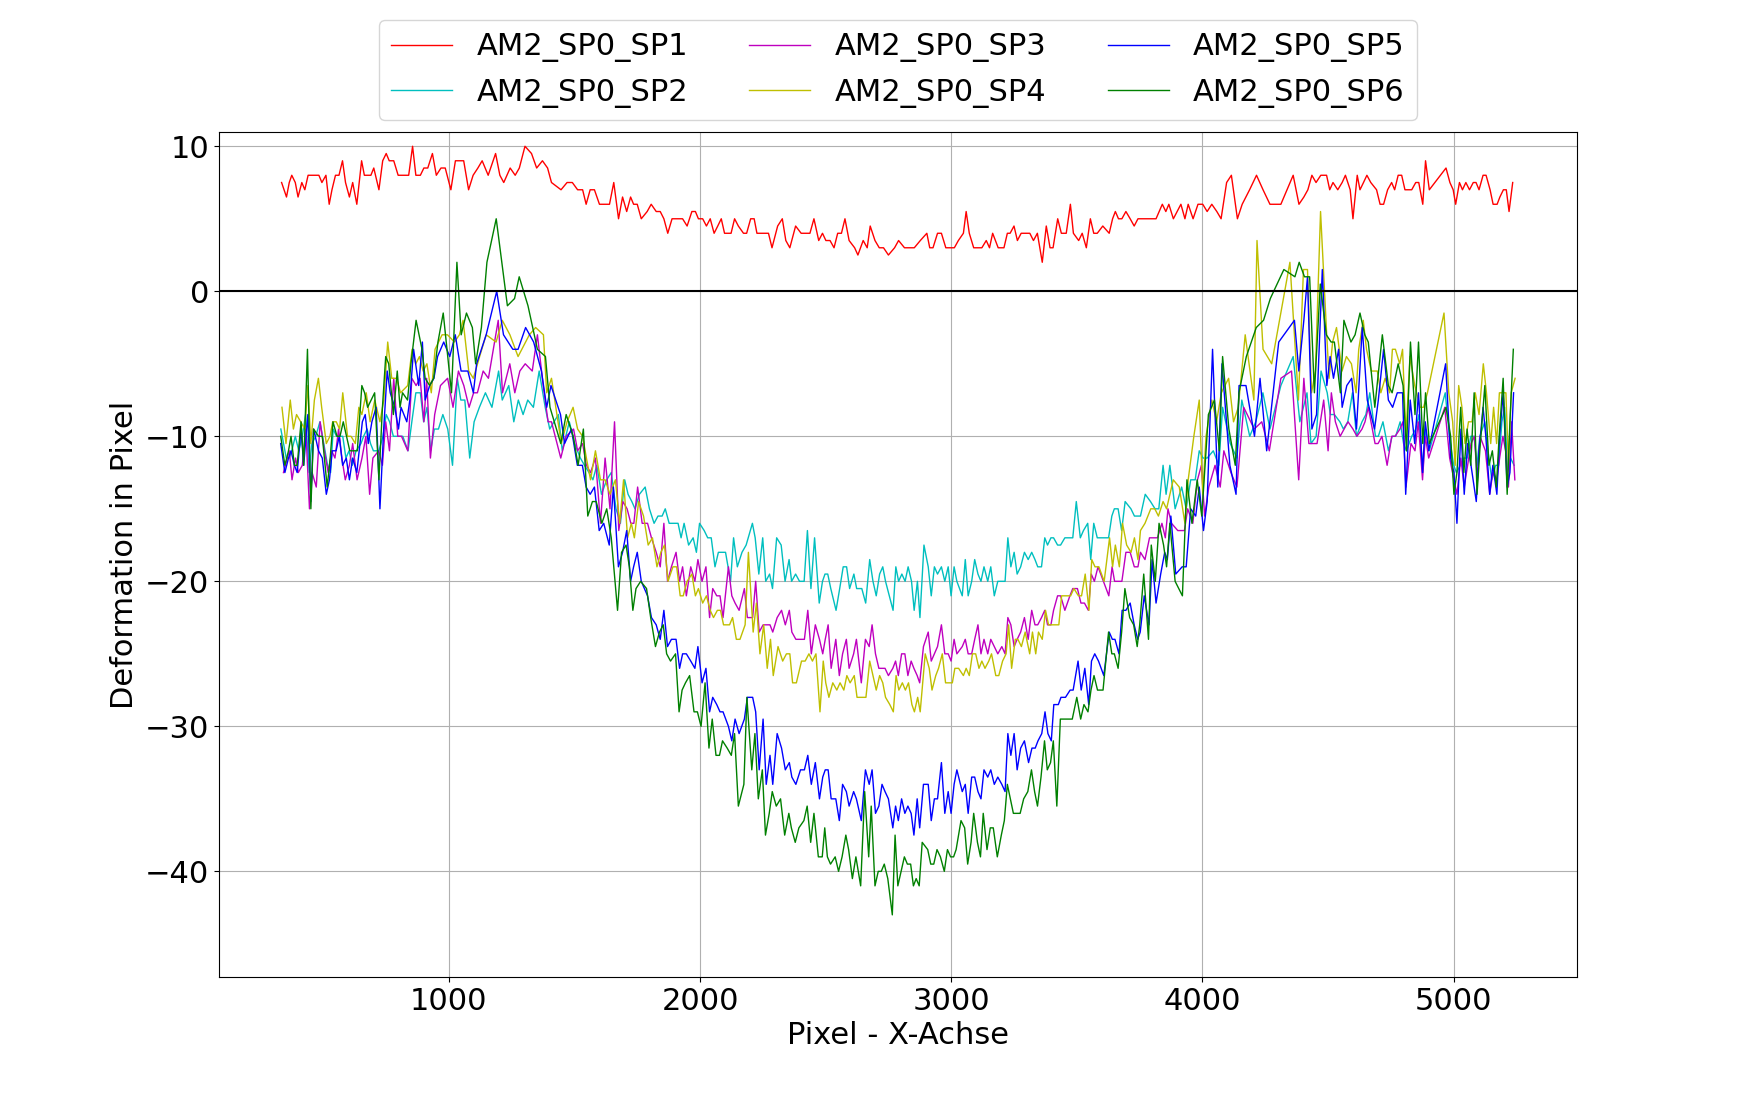
\includegraphics[width=0.95\textwidth]{images/am2_all_defos.png}
  \caption{Sechs Deformationsstufen bei einem AM Bauteil von 0 bis 2500 nm}
  \label{fig:am_defos}
\end{figure}

\begin{figure}[H]
  \centering
  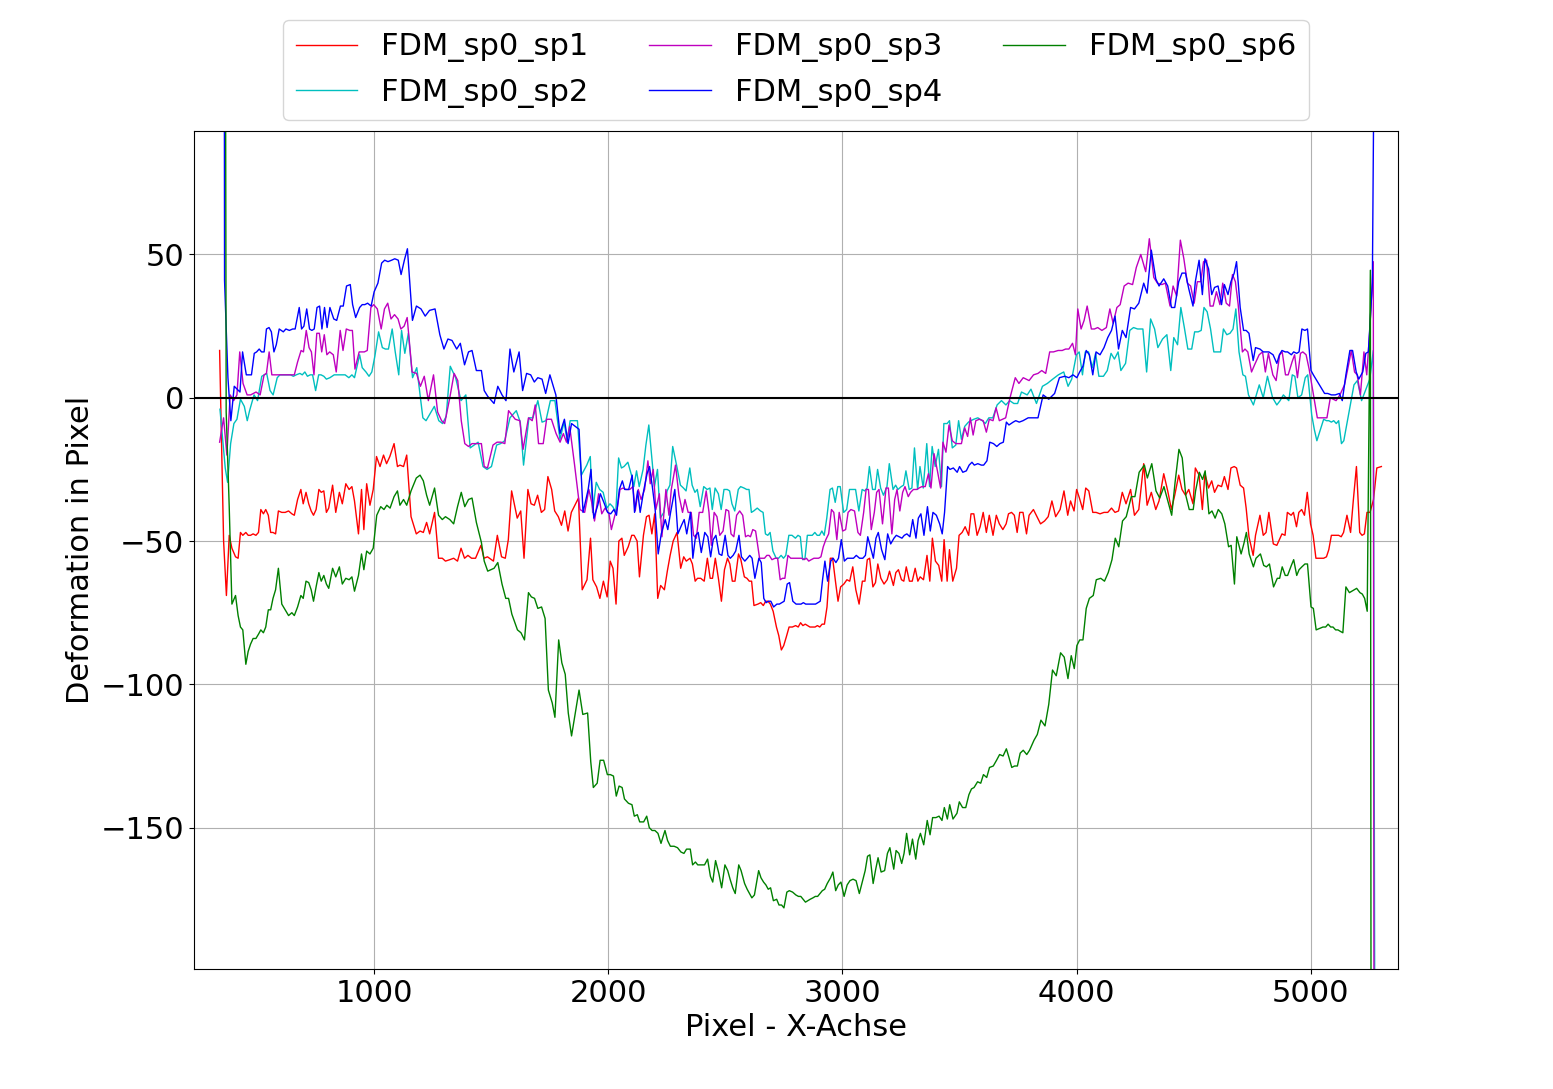
\includegraphics[width=0.95\textwidth]{images/fdm2_all_defos.png}
  \caption{Fünf Deformationsstufen bei einem FDM Bauteil von 0 bis 250 nm}
  \label{fig:fdm_defos}
\end{figure}

\section{Beurteilung der Ergebnisse}

Grundsätzlich kann mithilfe der Methodik die Deformation erkannt und verglichen 
werden.
Dennoch ist die Deformationserkennung noch nicht perfekt. 
Fehler im Stitching Prozess führen zu starken Änderungen in der Deformationserkennung. 
Wie in Abbildung \ref{fig:errors} zu sehen ist, kann sich die Breite des Bauteils 
zwischen zwei Spannungsstufen unterscheiden. Er ist erkennbar, dass der Rand der einen 
Kontur, repräsentiert durch die magenta gefärbte Linie, immer größer ist als 
der Rand der anderen Kontur, hier in blau dargestellt.
Dieser Versatz entsteht, weil beim Stitching eine Transformation verwendet wurde die sich 
um wenige Pixel unterscheidet. Dadurch wächst auch die erkannte Deformationen.
Aus diesem Grund existieren in den Abbildungen \ref{fig:am_defos} und \ref{fig:fdm_defos}
Linien die nicht dem erwarteten Verhalten entsprechen. 
In Abbildung \ref{fig:fdm_defos} zum Beispiel, sollte die Deformation zwischen den 
Spannungsstufen eins und zwei 
(in rot dargestellt) am kleinsten sein. Stattdessen liegt die Kurve mittig im Graph.
Genauso liegt die Deformation derselben 
Spannungsstufen bei dem Metallbauteil im Verhältnis zu den anderen zu hoch. 

\begin{figure}[H]
  \centering
  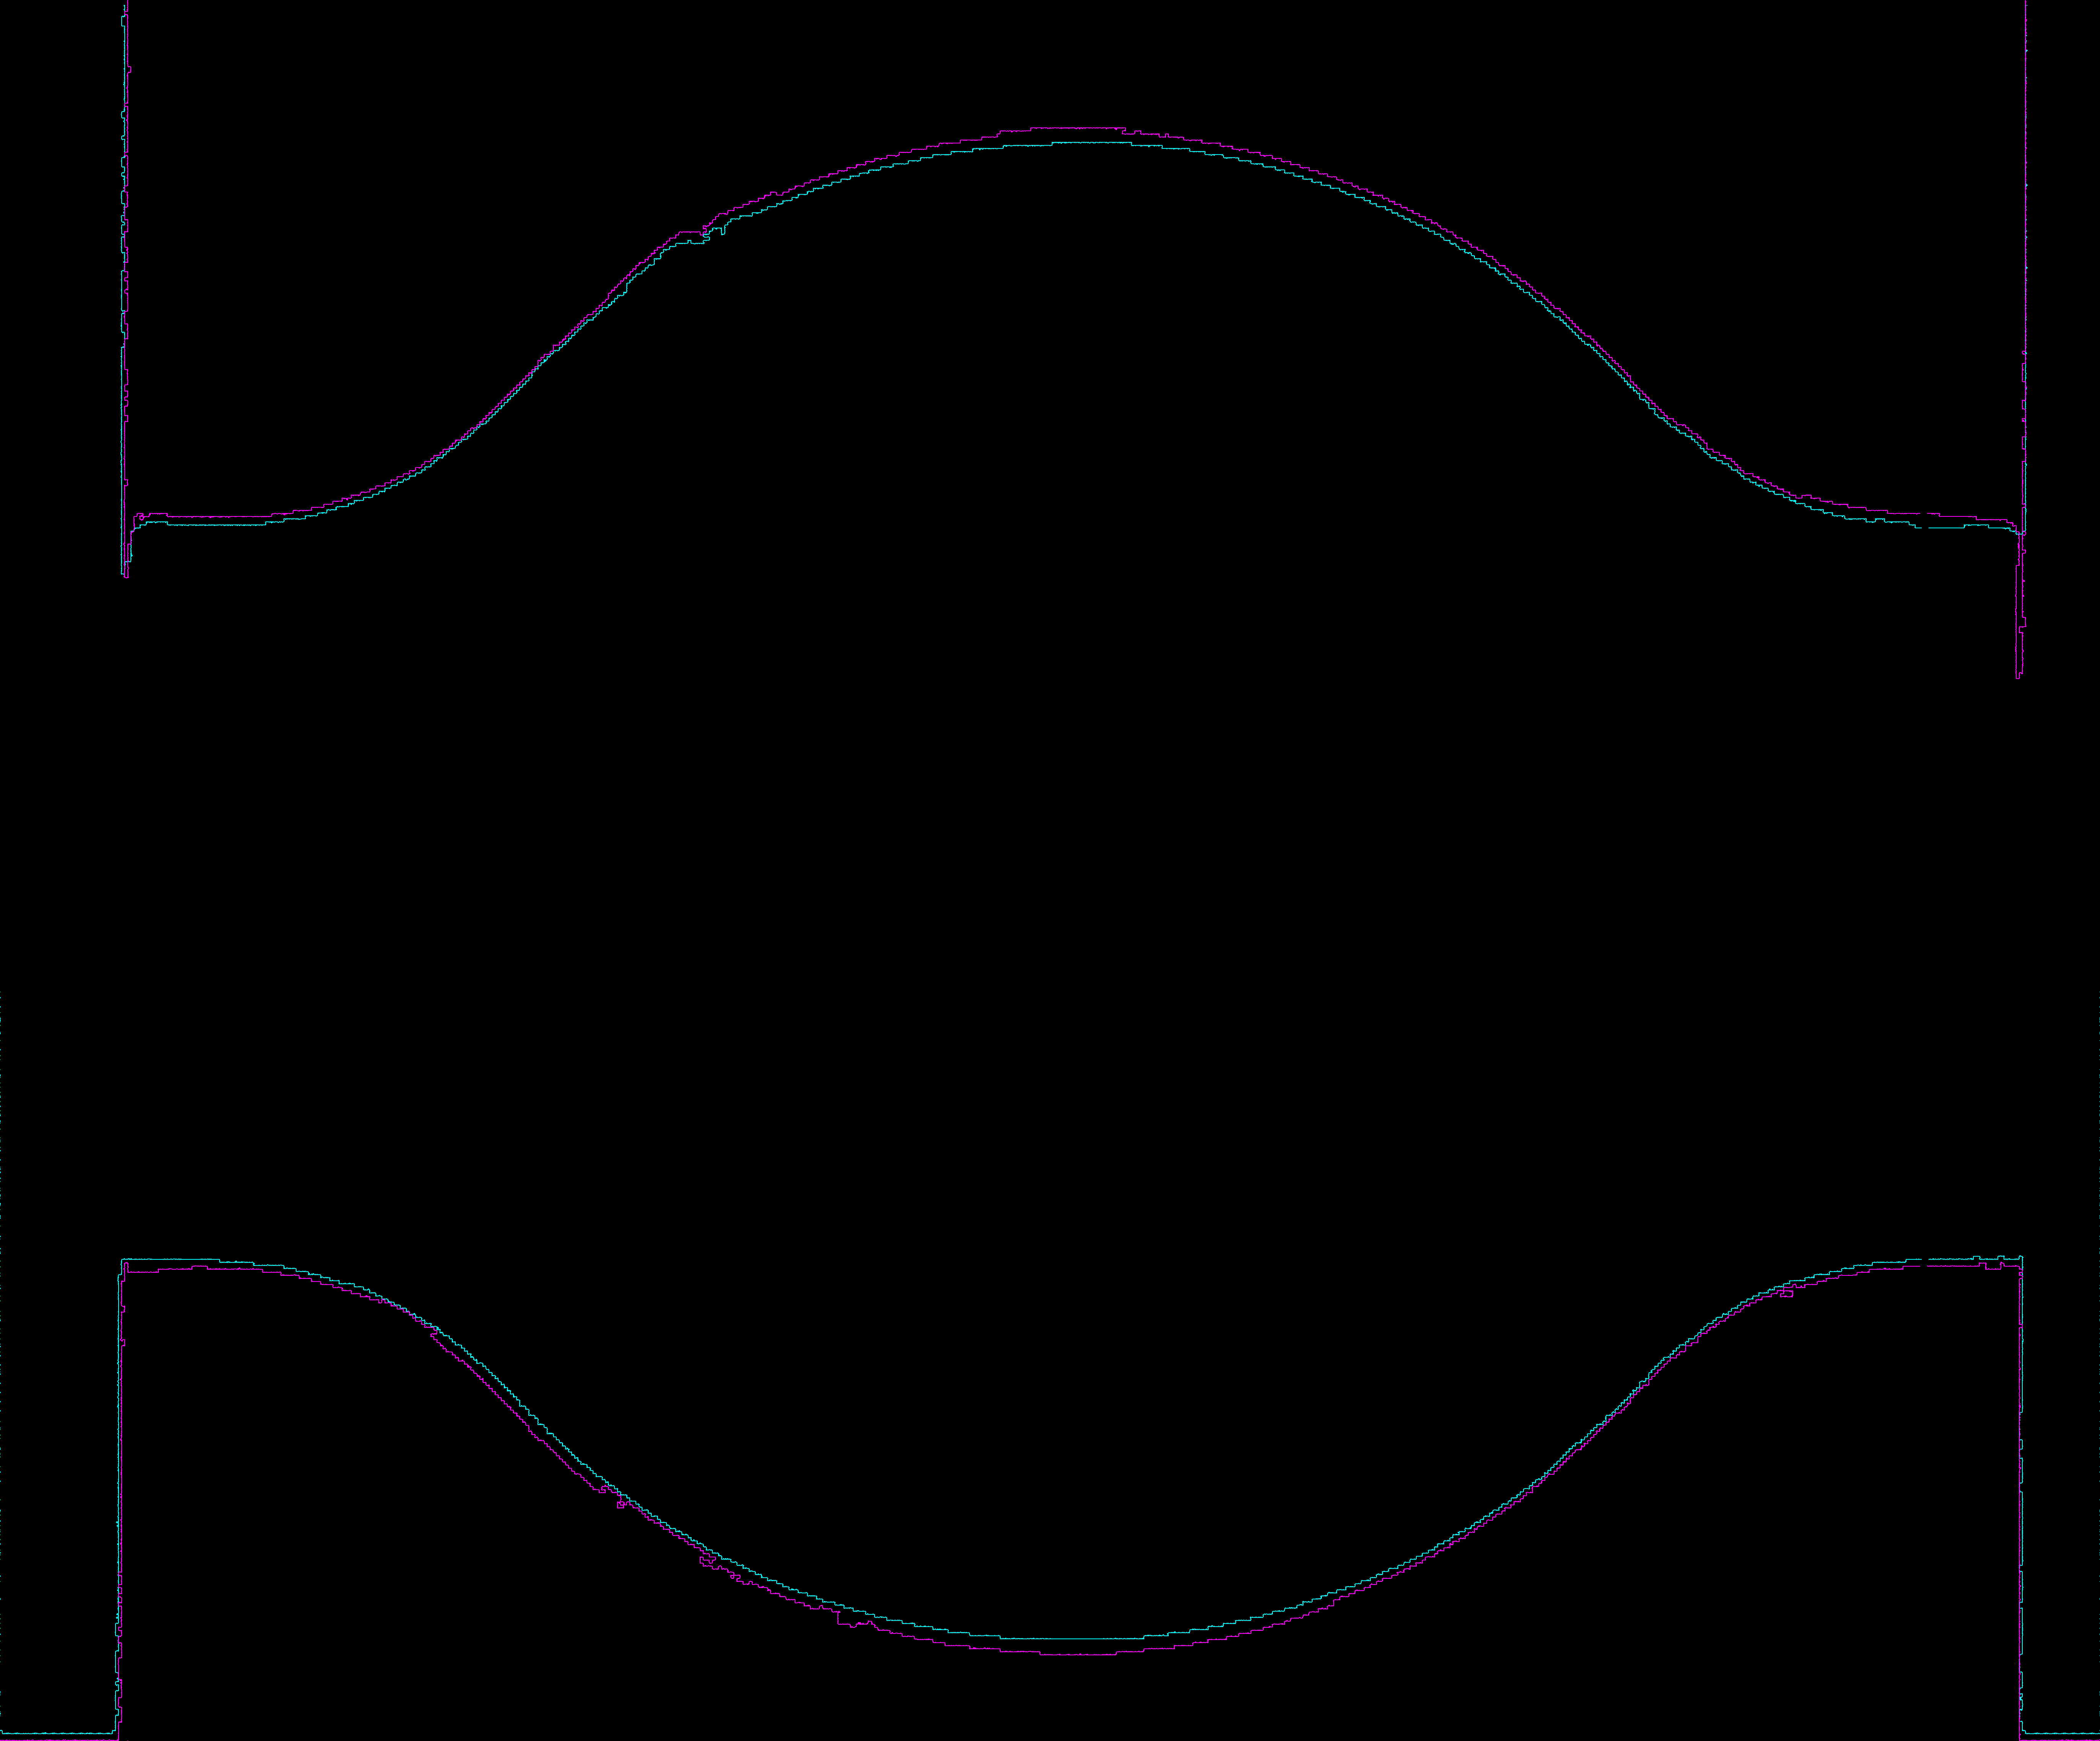
\includegraphics[width=0.95\textwidth]{images/FDM_sp0_stitched_FDM_sp1_stitched_0_0.png}
  \caption{Vergleich von Konturen aus nicht perfekt zusammengefügten Bildern. 
  Vergleich der Spannungsstufe null mit der Spannungsstufe eins eines FDM Demonstratorbauteils}
  \label{fig:errors}
\end{figure}
